\documentclass[a4paper,11pt]{article}

\usepackage[english,brazil]{babel}
\usepackage[utf8]{inputenc}
\usepackage{amsmath}
\usepackage{algorithm}
\usepackage{algpseudocode}
\usepackage{graphicx}
\usepackage{fancyhdr}
\usepackage{url}
\renewcommand{\baselinestretch}{1.5}
\usepackage{titling}
\usepackage{geometry}
\geometry{
 a4paper,
 left=25mm,
 right=25mm,
 top=1in,
 bottom=1in,
}
\usepackage{amsmath}
\usepackage{amssymb}
\usepackage{subfig}
\usepackage{multirow}
\usepackage[table]{xcolor}
\usepackage[backend=bibtex,style=ieee,sorting=none]{biblatex}
\bibliography{bibliography.bib}

\newcolumntype{C}{>{\centering\arraybackslash}p{1em}}

\title{\textbf{Tracking e Localização para Robôs Diferenciais Jogadores de Futebol}}

\author{Luis Guilherme Gomes Aguiar, Takashi Yoneyama\\
Instituto Tecnológico de Aeronáutica\\
São José dos Campos, SP, Brazil} %\\

\date{\today}

% ADD THE FOLLOWING COUPLE LINES INTO YOUR PREAMBLE
\let\OLDthebibliography\thebibliography
\renewcommand\thebibliography[1]{
  \OLDthebibliography{#1}
  \setlength{\parskip}{0pt}
  \setlength{\itemsep}{0pt plus 0.3ex}
}


% O DOCUMENTO COMEÇA AQUI
\begin{document}

\tableofcontents
\newpage

\maketitle

\section{Plano Inicial}
\textbf{1º bimestre (ago/set)}
\begin{itemize}
    \item Estudo de técnicas de filtragem estatística: Filtro de Kalman, Filtro de Kalman Extendido, Unscented Kalman Filter e Filtro de Partículas.
    \item Implementação dessas técnicas para um problema de localização genérico, utilizando linguagem de programação de alto nível.
\end{itemize}
\textbf{2º bimestre (out/nov)}
\begin{itemize}
    \item Estudo do modelo dinâmico do robô e dos sensores para modelar os sensores e a odometria.
\end{itemize}
\textbf{3º bimestre (dez/jan)}
\begin{itemize}
    \item Projeto de filtro estocástico
\end{itemize}

\section{Atividades realizadas}
\textbf{(ago/set/out)}
\begin{itemize}
    \item Estudo das técnicas de filtragem bayesianas Filtro de Kalman, Filtro de Kalman Extendido, Unscented Kalman Filter e Filtro de Partículas.
    \item Implementação dessas técnicas em problemas de localização genéricos, utilizando o software MATLAB, a fim de aplicar, compreender e comparar os algoritmos.
\end{itemize}
\textbf{(novembro)}
\begin{itemize}
    \item Modelamento estocástico do problema em questão, a partir da análise dos sensores e da dinâmica do robô.
\end{itemize}
\textbf{(dez/jan)}
\begin{itemize}
    \item Projeto de filtro estocástico para localização e tracking de bola e robôs no IEEE’s Very Small Size Soccer.
    \item Implementação em MATLAB
    \item Simulações, obtenção de estatísticas e avaliação de resultados e performance 
\end{itemize}

\section{Descrição do Problema}

Robótica móvel tem se se mostrado uma área de grande destaque no contexto atual, tanto pela abrangência e profundidade das pesquisas envolvidas quanto pelo rápido crescimento na indústria atualmente. A fim de incentivar e estimular pesquisas na área, foram criadas diversas competições nacionais e internacionais, como a RoboCup, mais famosa competição mundial criada em 1997 que tem como objetivo fomentar o avanço da robótica e inteligência artificial com o desafio de até 2050 criar um time de robôs humanoides capazes de ganhar de um time de humanos em uma partida de futebol.

Da mesma forma, vários desafios e competições foram criados com o objetivo de promover o avanço tecnológico em cada campo da robótica, como é o caso do IEEE’s Very Small Size Soccer (VSS). O VSS é uma liga de futebol de robôs autônomos mantida pela IEEE Robotics and Automation Society que consiste em uma partida de futebol disputada por três robôs diferenciais com dimensões máximas de 7,5x7,5x7,5cm. As informações da partida são captadas através de uma câmera acima do campo e processadas autonomamente por um computador, que a partir desses dados toma decisões de movimento aos robôs, enviadas por rádio, de forma a ganhar a partida.

Dessa forma, o problema deve ser modelado matematicamente e cada etapa processada, como a visão computacional, o controle, o cálculo de rotas, a estratégia a ser tomada e, inclusive, a localização do robô do nosso time, do time adversário, e da bola da partida.

Localização de robôs móveis é uma etapa fundamental no desenvolvimento de robótica. A dificuldade surge a partir do fato do mundo real não ser determinístico, mas ruidoso. Um exemplo disso são os dados dos sensores empregados. Nesse caso em particular fala-se da imagem da câmera; ou o modelo de movimento, que inclui uma diferença entre a ação comandada e a realizada pelos motores. Saber com acurácia e precisão a posição e a velocidade de robôs do próprio time e do time adversário é essencial nesse desafio, como requisitos para o desenvolvimento da estratégia de alto nível.

A abordagem estatística é amplamente aceita como a mais bem-sucedida para esse problema. Dessa forma, a observação e movimento são modelados como um processo de Markov. Os ruídos são variáveis aleatórias e os dados da odometria e visão são processados de forma a alcançar uma estimativa ótima da posição real do robô.

\section{Resultados}

\subsection{Introdução}

Como definido, o desafio lidado é o de se obter a posição e as velocidades linear e angular do robô diferencial na competição Very Small Size. A abordagem probabilística para esse problema consiste em tratar a posição do robô no campo em um dado tempo $t$ como um vetor de variáveis aleatórias $x_t$. O objetivo, portanto, é obter sua função distribuição de probabilidade ao longo de todo o espaço em questão.

O estado do robô $x_t$ deve englobar todas as grandezas necessárias para a sua localização e que tem impacto em seu estado futuro. E ainda, como desejado nesse problema, deve conter variáveis cinemáticas, como velocidades lineares e angulares.

Um robô interage com o ambiente através de sua percepção por meio de sensores e atuadores. Através de comandos de controle, incluindo sinais de referência tais como a velocidade linear, por exemplo, o robô se move, posiciona, e alcança a configuração de estado desejado.

A fim de empregar as técnicas de filtragem bayesianas amplamente usadas (\cite{P.Robotics} ,\cite{nonlinear_filtering}), como o filtro de Kalman ou o filtro de partículas, a dinâmica do robô é modelada através de duas equações estocásticas: a equação de movimento, que descreve como o estado varia no tempo como efeito de sua cinemática e controle (equação \eqref{basic_movement}), e a equação de observação, que descreve como se dá a observação obtida pelos sensores em função do estado (equação \eqref{basic_measurement}).


\begin{equation}
\label{basic_movement}
x_{t+1}=f(x_t,\epsilon_t)+u_t
\end{equation}
\begin{equation}
\label{basic_measurement}
z_t=h(x_t)+v_t
\end{equation}

 Na equação \eqref{basic_movement}, $\epsilon_t$ é o vetor de entradas de controle e $u_t$ um ruído de estado. Na equação \eqref{basic_measurement}, $v_t$ é também um ruído aleatório comum ao processo de observação pelo sensor.

Considerando as funções distribuição de probabilidade, a probabilidade do do estado estar em $x_t$, condicionado ao fato de estar em $x_{t-1}$ no instante $t-1$, é dada por $p(x_t |x_{t-1})$, enquanto a da observação é dada por $p(z_t |x_t)$. A ideia central por trás dos filtros bayesianos é obter uma distribuição a posteriori para o estado do robô, mesclando as informações dos passos de movimento e observação através de um algoritmo de filtragem. A distribuição desejada, incluindo a observação no instante, seria, portanto, $p(x_t |z_{1:t})$. As equações \eqref{bayes_filter1} e \eqref{bayes_filter2}, presentes em \cite{P.Robotics} e \cite{Simo_bayesianFiltering}, descrevem o filtro de Bayes para as hipóteses assumidas nas equações \eqref{basic_movement} e \eqref{basic_measurement}.

\begin{equation}
    \label{bayes_filter1}
    p(x_t|z_{1:t-1})=\int p(x_t|x_{t-1})\: \mathrm{d}x_{t-1}
\end{equation}

\begin{equation}
\label{bayes_filter2}
    p(x_t|z_{1:t})= \frac{p(z_t|x_t)p(x_t|z_{1:t-1})}{\int p(z_t|x_t)p(x_t|z_{1:t-1})\: \mathrm{d}x_{t-1}}
\end{equation}

\subsection{Filtros Bayesianos}

Para sistemas não lineares, como descritos pelas equações \eqref{basic_movement} e \eqref{basic_measurement}, o filtro de Bayes, em geral, é de difícil aplicação prática. Como observa-se na equação \eqref{bayes_filter1} a integral descrita pode ser de difícil cálculo ou até mesmo nem ter uma expressão analítica fechada. Contudo, existem diferentes técnicas e algoritmos que fornecem aproximações satisfatórias para esse filtro, com mudanças características de hipóteses, eficiência computacional, precisão da aproximação e facilidade de implementação. Cada técnica resulta em diferentes distribuições de probabilidade finais para o estado calculado, dependendo das hipóteses assumidas para cada implementação. Com isso, foi realizado o estudo das técnicas mundialmente mais conhecidas e empregadas em localização e tracking de robô móvel, como o filtro de Kalman, e suas extensões não lineares, como o EKF e UKF, além do filtro não paramétrico mais empregado: filtro de partículas.

O filtro de Kalman é a técnica mais conhecida e já estudada de filtragem estocástica(\cite{P.Robotics} e \cite{Optimal_Filtering}). Ele é uma solução ótima para o cálculo da distribuição posteriori em sistemas lineares sujeitos a ruídos brancos graussianos. Para esses sistemas, a resposta a uma entrada gaussiana (ou normal) é também gaussiana. Logo, nesse algoritmo, pode-se representar a distribuição de cada estado por seus parâmetros média ($\mu_t$) e covariância ($\Sigma_t$). Sendo $u_t\sim N(0,Q_t)$ e $v_t\sim (0,R_t)$.

\begin{equation}
    \label{linear_movement}
    x_t=A_t x_{t-1} + B_t\varepsilon_t + u_t
\end{equation}
\begin{equation}
    \label{linear_measurement}
    z_t = C_t x_t + v_t
\end{equation}

\selectlanguage{brazil}
\begin{algorithm} 
\caption{Filtro de Kalman, extraído de  [\cite{P.Robotics}p.42]}
\label{alg1}
\begin{algorithmic}[1]
\Function {Filtro de Kalman}{$\mu_{t-1}, \Sigma_{t-1}, u_t, z_t$}
\State \textbf{Predição}
\State $\overline{\mu_t} = A_t \mu_{t-1} + B_t\varepsilon_t + u_t$
\State $\overline{\Sigma_t} = A_t\Sigma_{t-1}A_t^{T}+Q_t$
\State \textbf{Atualização}
\State $K_t=\overline{\Sigma_t}C_t^{T}(C_t\overline{\Sigma_t}C_t^{T}+R_t)^{-1}$
\State $\mu_t = \overline{\mu_t} + K_t(z_t-C_t\overline{\mu_t})$
\State $\Sigma_t=(I-K_t C_t)\overline{\Sigma_t}(I-K_t C_t)^{T}+K_t R_t K_t^{T}$
\EndFunction
\end{algorithmic}
\end{algorithm}

O filtro de Kalman possui um custo computacional muito baixo, sendo, portanto, muito rápido e de boa aplicação para sistemas que demandam filtragem em tempo real. Sua desvantagem é sua limitação, sendo restrito a sistemas lineares, o que constitui casos bem restritos em problemas práticos de mundo real.

O filtro de Kalman extendido \cite{Optimal_Filtering} é uma versão não linear do filtro de Kalman que se baseia na linearização das equações de atualização e de medida em torno do ponto de maior probabilidade, e a partir dessas linearizações aplica-se o filtro de Kalman convencional.

A partir de um sinal gaussiano para $x_{t-1}$, aplica-se as equações não lineares, como descritas em (\ref{basic_movement}) e (\ref{basic_measurement}). O sinal seria então deformado por essa propagação. Aplica-se uma expansão de primeira ordem do polinômio de Taylor no ponto de concentração de maior probabilidade, e a seguir, a partir da função linear obtida, o filtro de Kalman. O processo é ilustrado na figura \ref{linearization}.

\begin{figure}[!t]
\centering
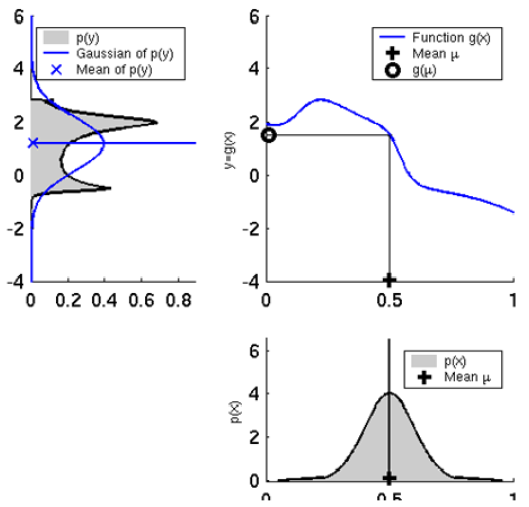
\includegraphics[width = 0.6\textwidth]{LinearizacaoEKF.png}
\DeclareGraphicsExtensions.
\caption{Linearização pelo EKF}
\label{linearization}
\end{figure}

Observa-se que a distribuição posteriori é uma gaussiana, apesar da forma da distribuição final desejada, $p(x_t |z_{1:t})$, não ser necessariamente uma gaussiana. O resultado obtido é então uma aproximação na forma de gaussiana. Como pode ser observado pela matemática da técnica, a eficiência dessa aproximação pode ser limitada pelo fato do sistema e as equações de atualização ou medida serem altamente não lineares, ou ainda por uma original alta variância nos sinais filtrados. O custo computacional do algoritmo é muito baixo, tal como o filtro de Kalman.

O algoritmo do filtro de Kalman pode ser adaptado para essa linearização via expansão de Taylor. Com isso, o algoritmo seria o mesmo, com a particularidade de que $A_t$ seria a jacobiana de $f$ calculada no ponto $\mu_{t-1}$, enquanto $B_t$ seria a jacobiana de $h$ calculada no ponto $\overline{\mu_t}$.
\begin{equation}
    A_t = \frac{\partial f}{\partial x}(\mu_{t-1})
\end{equation}
\begin{equation}
    C_t = \frac{\partial h}{\partial x}(\overline{\mu_t})
\end{equation}

Como abordado em \cite{unscented_filtering} e \cite{ukf}, o \textit{Unscented Kalman Filter}, ou UKF, é outra extensão não linear do filtro de Kalman com o mesmo princípio de linearizar uma transformação de um vetor de variáveis aleatórias gaussianas. A aproximação utilizada é baseada na \textit{unscented transformation}, e consiste em extrair deterministicamente pontos específicos, chamados \textit{sigma points}, da entrada gaussiana e então passá-los pela função de atualização não linear $f$. As médias e covariâncias são extraídas com pesos em relação a esses \textit{sigma points}.

O UKF, apesar de ser um algoritmo de compreensão complexa, possui algumas vantagens em relação ao EKF. A primeira e imediata é a ausência da necessidade de se calcular as derivadas parciais para as jacobianas presentes no EKF, o que pode ser difícil de determinar analiticamente para alguns casos. A segunda vantagem é o desempenho em precisão ser melhor ou igual ao do EKF, principalmente nos casos de alta não linearidade e variância alta na entrada. No geral o UKF é ligeiramente mais lento do que o EKF, mas ainda assim possui um custo computacional baixo. Vale lembrar que o UKF, assim como o filtro de Kalman extendido, representa as distribuições posterioris como gaussianas que melhor aproximam a distribuição pretendida $p(x_t |z_{1:t})$, tendo, portanto, dificuldades em representar distribuições multimodais. 

O filtro de partículas é, dessa forma, uma solução a essa limitação pela sua natureza não paramétrica (\cite{monte_carlo_localization} e \cite{particle_filter}). O filtro busca, primeiramente, estimar a distribuição de probabilidade $p(x_t|x_{t-1})$ propagando várias amostras, denominadas partículas, do estado $x_{t-1}$ através da equação de estado. Após a obtenção de várias partículas propagadas, a nova etapa, denominada de filtragem, está em corrigir as posições de tais amostras com os pesos dados pela equação \eqref{weight}. O processo é repetido gerando-se novas partículas através de reamostragem. A ideia central do filtro é explorar a dualidade entre distribuições de probabilidade e um conjunto de amostras geradas por essa função de distribuição. Além disso, qualquer expectativa da distribuição sobre o espaço pode ser calculado pelo método de Monte Carlo, que segue na equação \eqref{montecarlo}. Na equação \eqref{weight}, $\eta$ é uma constante de proporcionalidade usada para normalizar o valor dos pesos.

\begin{equation}
\label{weight}
w_t^{[m]} = \eta w_{t-1}^{[m]}p(z_t|x_t)
\end{equation}
\begin{equation}
\label{montecarlo}
\small{
\left[\displaystyle\sum_{m=1}^{M} w_t^{[m]}\right]^{-1} \displaystyle\sum_{m=1}^{M} {g(x_t^{[m]})w_t^{[m]}} \xrightarrow[]{M \rightarrow \infty} \int_A \mathrm{g(x_t)p(x_t|z_{1:t})}\,\mathrm{d}x_t}
\end{equation}

Nas equações, $w_t^{[m]}$  é o peso para a $m$-ésima partícula no instante $t$, $M$ é a quantidade de partículas, e $g(x)$ uma função mensurável qualquer. Com o filtro de partículas, a distribuição posteriori desejada pode ser bem aproximada mesmo que seja multimodal, desde que tenhamos um número de partículas suficientemente grande. Essa é a principal vantagem do filtro de partículas. Sua maior desvantagem é o custo computacional, que pode crescer significativamente com o aumento da quantidade de partículas.

\subsection{Projeto e alterações}

A ideia inicialmente pretendida para o projeto era a de estender o estado na filtragem da posição dos robôs do nosso time de VSS, acrescentando suas velocidades linear e angular. Um modelo de filtro e sua implementação no MATLAB já foram feitos antes por outro integrante do grupo, contudo só incluía as entradas necessárias para sua localização espacial, coordenadas planas $x$ e $y$ e ângulo de miragem $\psi$ do robô. Os dados de velocidades linear e angular ainda eram ruidosas, e a ideia era incluir tais grandezas no filtro estocástico. Contudo, o filtro não seria tão eficiente para essa finalidade, e a solução para diminuir o ruído nos valores de controle $v$ e $w$ foi um filtro passa baixas.

Outra ideia para minimizar tal incerteza, ainda a ser implementada, e que é muito usada em robótica, é ajustar os valores de controle linearmente. Dessa forma, se $[v,w]$ são os valores de controle comandados, procura-se determinar empiricamente parâmetros $\xi$ e $\eta$ de forma que $[\xi v,\eta w]$ se aproxima mais aos reais valores de controle.

O projeto focou-se então em implementar os algoritmos de tracking dos robôs adversários e da bola, utilizando os filtros bayesianos estudados e incluindo as velocidades linear e angular no estado dinâmico. Nesse caso, o filtro ofereceria uma boa estimativa sobre essas variáveis, visto que as entradas de controle do adversário são desconhecidas, e a priori não temos nenhuma informação sobre suas variáveis dinâmicas $v$ e $w$.

\subsection{Modelo Matemático}

No tracking do robô, uma vez que as entradas de controle são desconhecidas, as equações de atualização e medida serão da forma:

\begin{equation}
\label{tracking_motion}
x_t=f(x_{t-1})+M_t u_t
\end{equation}

\begin{equation}
\label{tracking_measurement}
z_t=h(x_t)+\vartheta_t
\end{equation}

O estado completo do robô diferencial pode ser descrito por suas coordenadas cartesianas planas em função do tempo, $x_t$ e $y_t$, por seu ângulo de orientação em função do tempo $\psi_t$, definido a partir do semi-eixo positivo das abcissas com sentido trigonométrico, e pelas velocidades linear $v_t$ e angular $w_t$. Dessa forma, o modelo contínuo de atualização na posição é dado pela equação \eqref{modelo_continuo}.

\begin{equation}
    \label{modelo_continuo}
    \begin{bmatrix} \dot{x_t} \\ \dot{y_t} \\ \dot{\psi_t} \\ \dot{v_t} \\ \dot{w_t}
    \end{bmatrix}
    =
    \begin{bmatrix} v_t \cos{\psi_t} \\ v_t \sin{\psi_t} \\ w_t \\ a \\ \alpha
    \end{bmatrix}
\end{equation}

O modelo discreto de movimento é obtido a partir da integração da equação \eqref{modelo_continuo} no intervalo $[(t-1),t]$. O intervalo de tempo entre dois instantes consecutivos é constante $T$. Para as atualizações de $x$ e $y$ considera-se um movimento uniforme de velocidades constantes $v_{t-1}$ e $w_{t-1}$, já que a integração com acelerações linear e angular não possui uma expressão analítica simples, não sendo, portanto, adequada para ser incluída na formulação do EKF, e além disso os ruídos aditivos atenuam parcialmente essa falha de modelo. Por último, as acelerações serão inseridas no modelo dinâmico como valores aleatórios inclusos no ruído gaussiano aditivo $u_t \sim N(0,Q)$. No ruído da observação temos também $v_t \sim N(0,R)$.

\begin{equation}
\label{update_equation}
\begin{bmatrix} x_t \\ y_t \\ \psi_t \\ v_t \\ w_t \end{bmatrix}
= \begin{bmatrix}
x_{t-1}+\frac{2v_{t-1}}{w_{t-1}} \sin{\left(\frac{w_{t-1}T}{2}\right)}\cos{\left(\psi_{t-1}+\frac{w_{t-1}T}{2}\right)} \\
y_{t-1}+\frac{2v_{t-1}}{w_{t-1}} \sin{\left(\frac{w_{t-1}T}{2}\right)}\sin{\left(\psi_{t-1}+\frac{w_{t-1}T}{2}\right)} \\
\psi_{t-1}+w_{t-1}T \\ v_{t-1} \\ w_{t-1} \end{bmatrix} +
\begin{bmatrix} 1 & 0 & 0 & 0 & 0 \\ 0 & 1 & 0 & 0 & 0 \\ 0 & 0 & 1 & 0 & \frac{T^2}{2} \\ 0 & 0 & 0 & T & 0 \\ 0 & 0 & 0 & 0 & T \end{bmatrix}
\begin{bmatrix} u_x \\ u_y \\ u_{\psi} \\ a \\ \alpha \end{bmatrix}
\end{equation}

\begin{equation}
    \label{observation}
    z_t = 
    \begin{bmatrix} x_t \\ y_t \\ \psi_t \end{bmatrix}
    +
    \begin{bmatrix} \vartheta_x \\ \vartheta_y \\ \vartheta_{\psi} \end{bmatrix}
\end{equation}

O modelo para o tracking da bola segue a mesma lógica, contudo não temos mais uma orientação. A bola possui liberdades de movimento independentes em $x$ e $y$.

\begin{equation}
    \begin{bmatrix} x_t \\ y_t \\ v_{x,t} \\ v_{y,t} \end{bmatrix}
    =
    \begin{bmatrix} 1 & 0 & T & 0 \\ 0 & 1 & 0 & T \\ 0 & 0 & 1 & 0 \\ 0 & 0 & 0 & 1 \end{bmatrix}
    \begin{bmatrix} x_{t-1} \\ y_{t-1} \\ v_{x,t-1} \\ v_{y,t-1} \end{bmatrix}
    +
    \begin{bmatrix} 1 & 0 & \frac{T^2}{2} & 0 \\ 0 & 1 & 0 & \frac{T^2}{2} \\ 0 & 0 & T & 0 \\ 0 & 0 & 0 & T \end{bmatrix}
    \begin{bmatrix} \beta_x \\ \beta_y \\ a_x \\ a_y \end{bmatrix}
\end{equation}

\begin{equation}
    z_t = \begin{bmatrix} x_t \\ y_t \end{bmatrix}
\end{equation}

\subsection{Simulações e Estatísticas}

Para implementar os modelos de tracking explicitados, foi empregado o filtro de Kalman extendido. A técnica serviu bem aos modelos, já que não temos nenhuma equação de atualização altamente não linear que prejudique a aproximação do filtro, e além disso o EKF é relativamente fácil de aplicar nesse caso e tem o custo computacional conhecidamente muito baixo.

Por enquanto, o filtro foi implementado apenas em MATLAB e extraímos a simulação considerando tempo total de $100s$ e intervalo de $\frac{1}{30}s$ entre cada iteração. Os valores empregados para $Q$ e $R$ seguem na tabela \ref{covariancias1}.

\begin{table}[!t]
\caption{Covariâncias - Tracking adversário}
\label{covariancias1}
\centering
% Some packages, such as MDW tools, offer better commands for making tables
% than the plain LaTeX2e tabular which is used here.
\begin{tabular}{c} 
$Q = \begin{bmatrix} $0.15$ & $0$ & $0$ & $0$ & $0$ \\ $0$ & $0.15$ & $0$ & $0$ & $0$\\ $0$ & $0$ & $0.01$ & $0$ & $0$ \\ $0$ & $0$ & $0$ & $3$ & $0$ \\ $0$ & $0$ & $0$ & $0$ & $5$
\end{bmatrix}$\\
$R = \begin{bmatrix} $0.15$ & $0$ & $0$ \\ $0$ & $0.15$ & $0$ \\ $0$ & $0$ & $0.01$\end{bmatrix}$\\
\end{tabular}
\end{table}

Os resultados gráficos para a simulação do tracking do robô adversário podem ser vistos na figura \ref{estatisticas_adversario}. A figura \ref{trajetorias} mostra as trajetórias real, estimada e a calculada pela observação apenas. As figuras \ref{RSE-x}, \ref{RSE-y}, \ref{RSE-psi}, \ref{RSE-v} e \ref{RSE-w} mostram o erro quadrático da estimativa em relação ao real ao longo da simulação para os valores de $x$, $y$, $\psi$, $v$ e $w$, respectivamente.

%FIGURAS

% trajetórias e erro em x
 \begin{figure}[!ht]
    \subfloat[Trajetórias - Simulação\label{trajetorias}]{%
      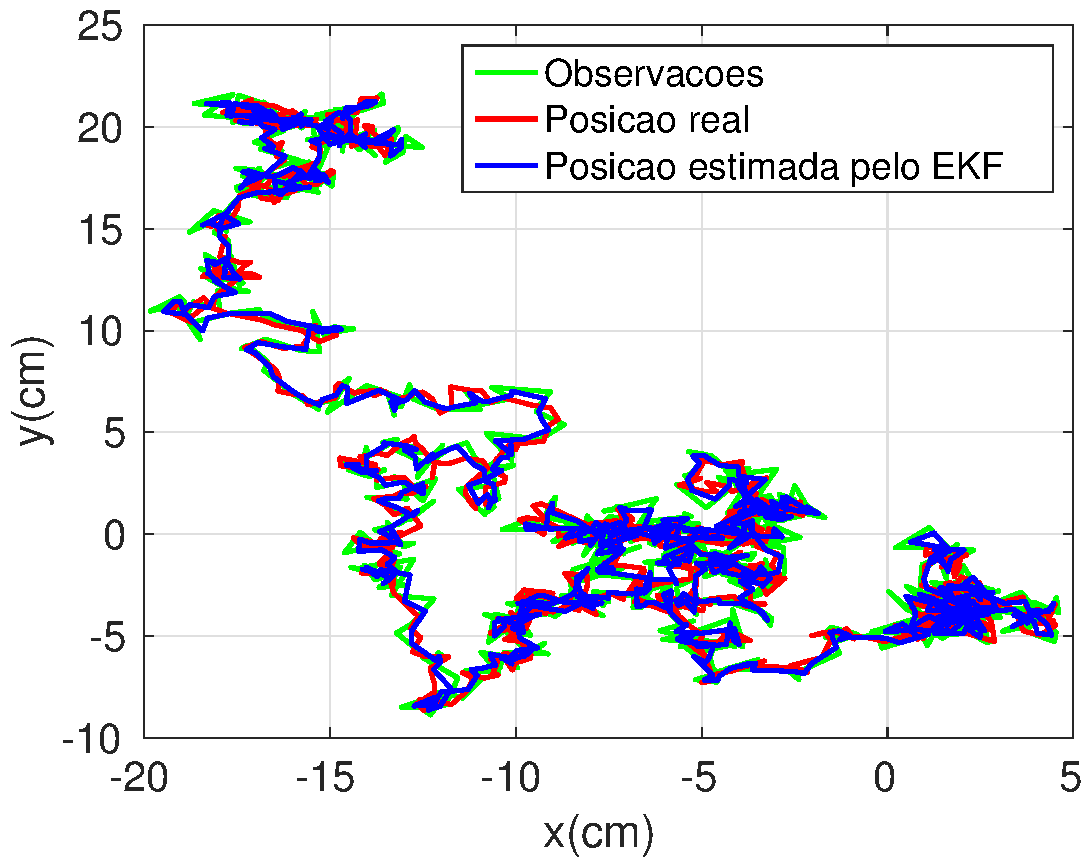
\includegraphics[width=0.45\textwidth]{trajetorias.pdf}
    }
    \hfill
    \subfloat[RSE-$x$\label{RSE-x}]{%
      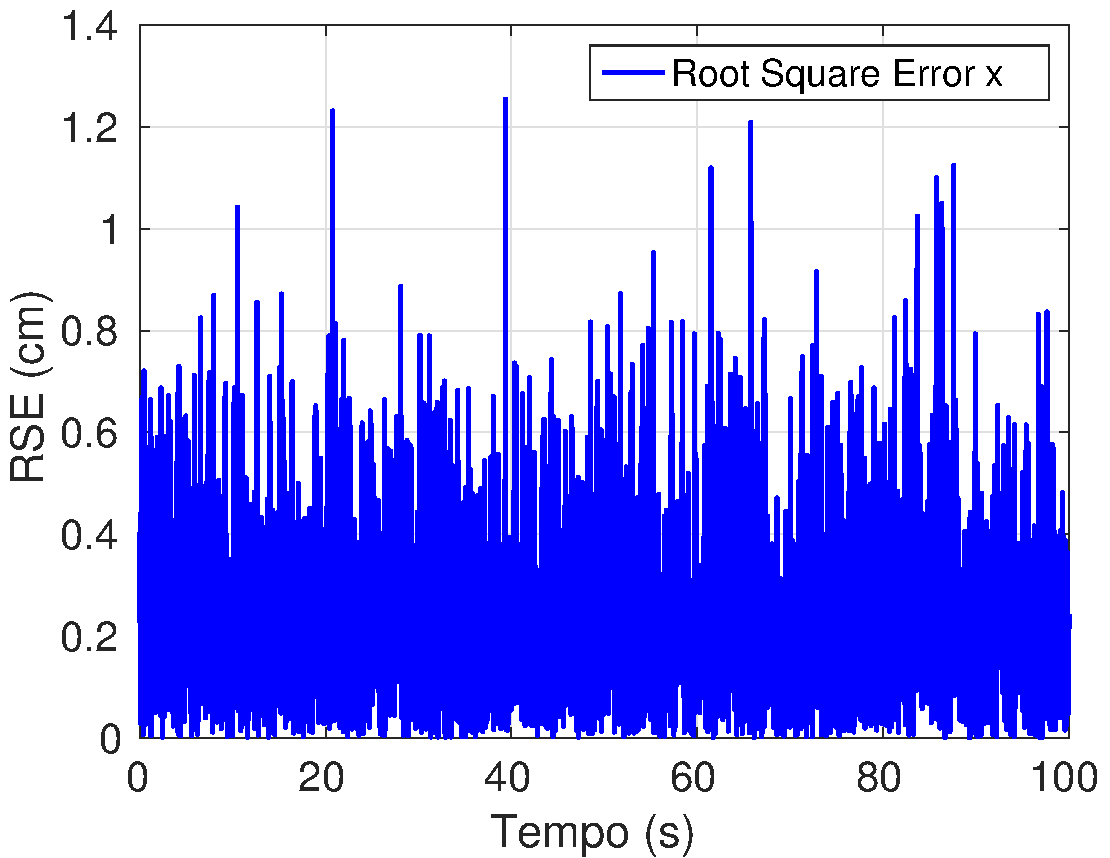
\includegraphics[width=0.45\textwidth]{RSE-x.pdf}
    }
    \hfill
%    \caption{Trajetórias e Root Square Error em $x$ - Tracking adversário}
%    \label{trajetorias-errox}
%  \end{figure}
% erro em y e psi
% \begin{figure}[!ht]
    \subfloat[RSE-$y$\label{RSE-y}]{%
      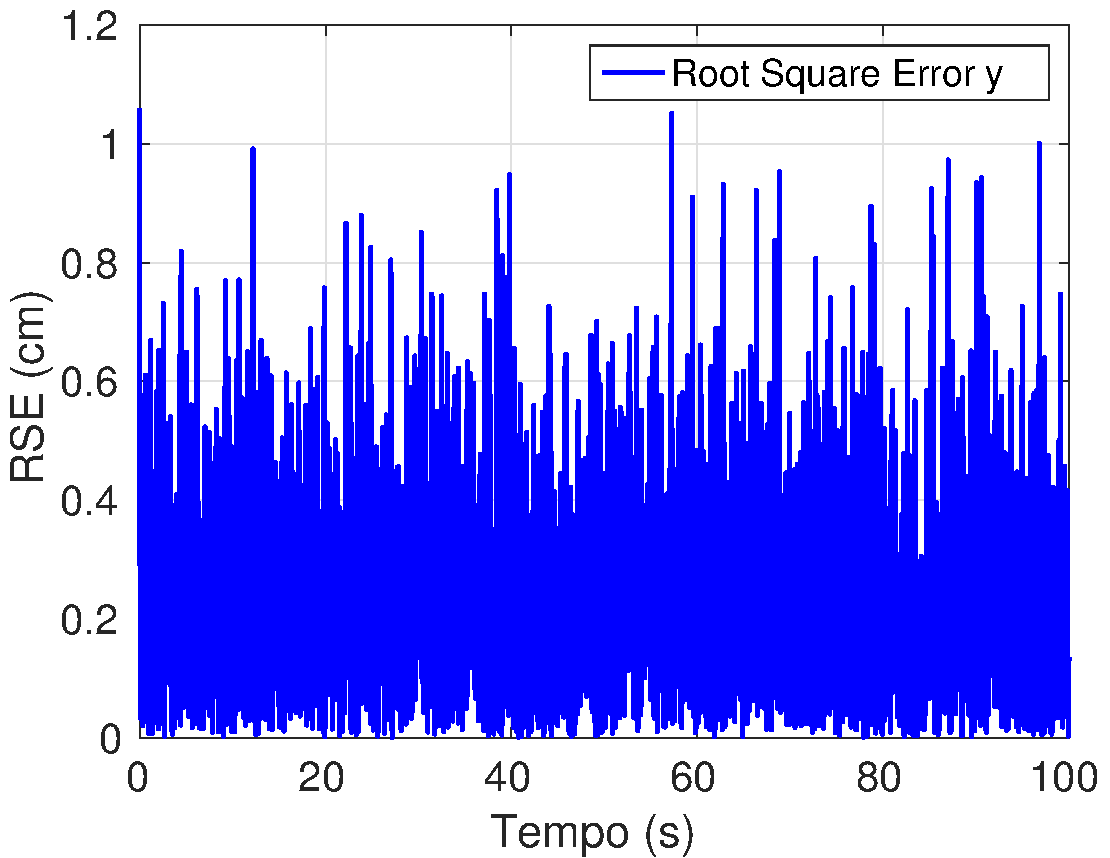
\includegraphics[width=0.45\textwidth]{RSE-y.pdf}
    }
    \hfill
    \subfloat[RSE-$\psi$\label{RSE-psi}]{%
      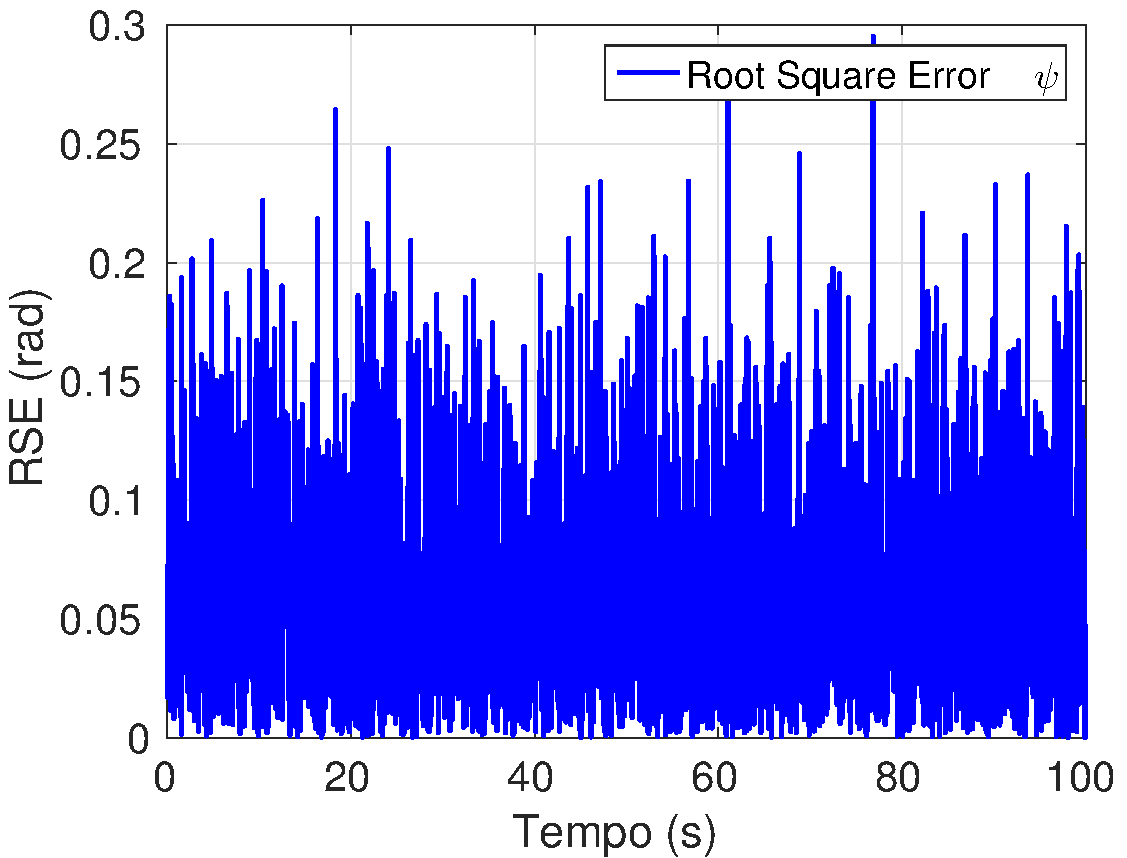
\includegraphics[width=0.45\textwidth]{RSE-psi.pdf}
    }
    \hfill
%    \caption{Root Square Error em $y$ e $\psi$ - Tracking adversário}
%    \label{erros_ypsi}
%  \end{figure}
  % erro em v e w
%  \begin{figure}[!ht]
    \subfloat[RSE-$v$\label{RSE-v}]{%
      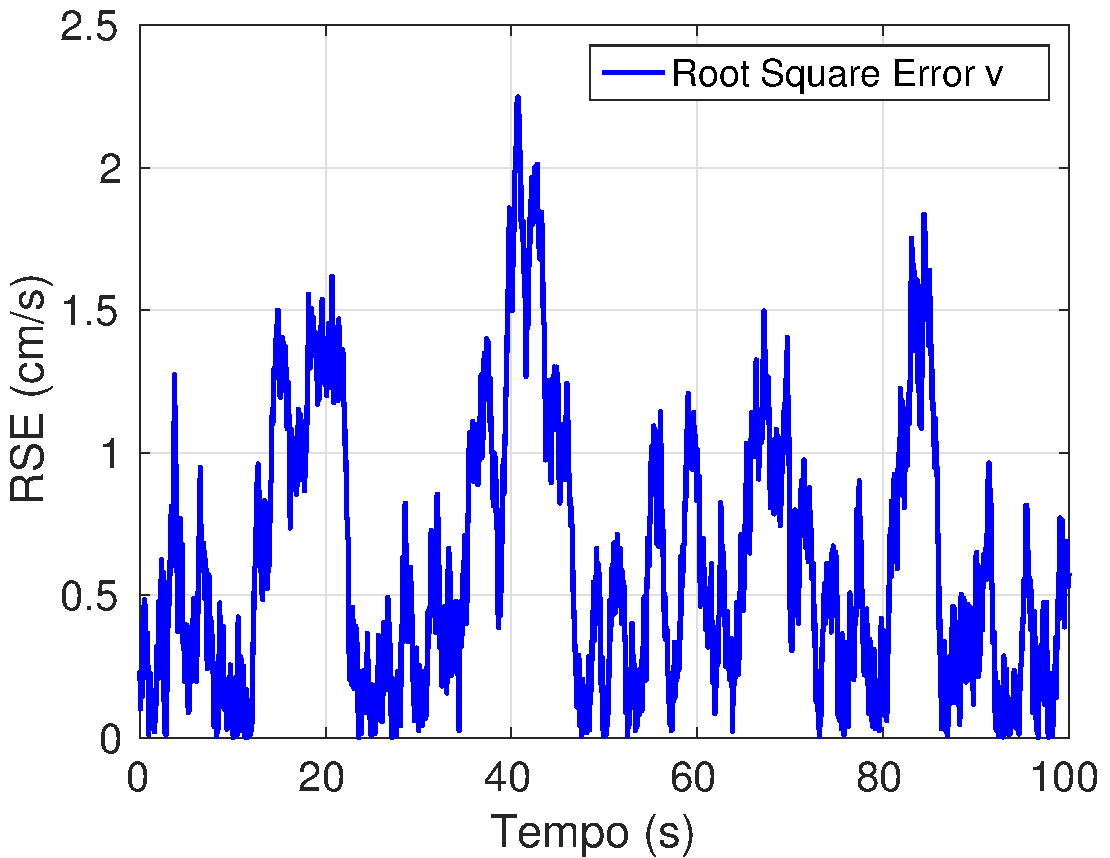
\includegraphics[width=0.45\textwidth]{RSE-v.pdf}
    }
    \hfill
    \subfloat[RSE-$w$\label{RSE-w}]{%
      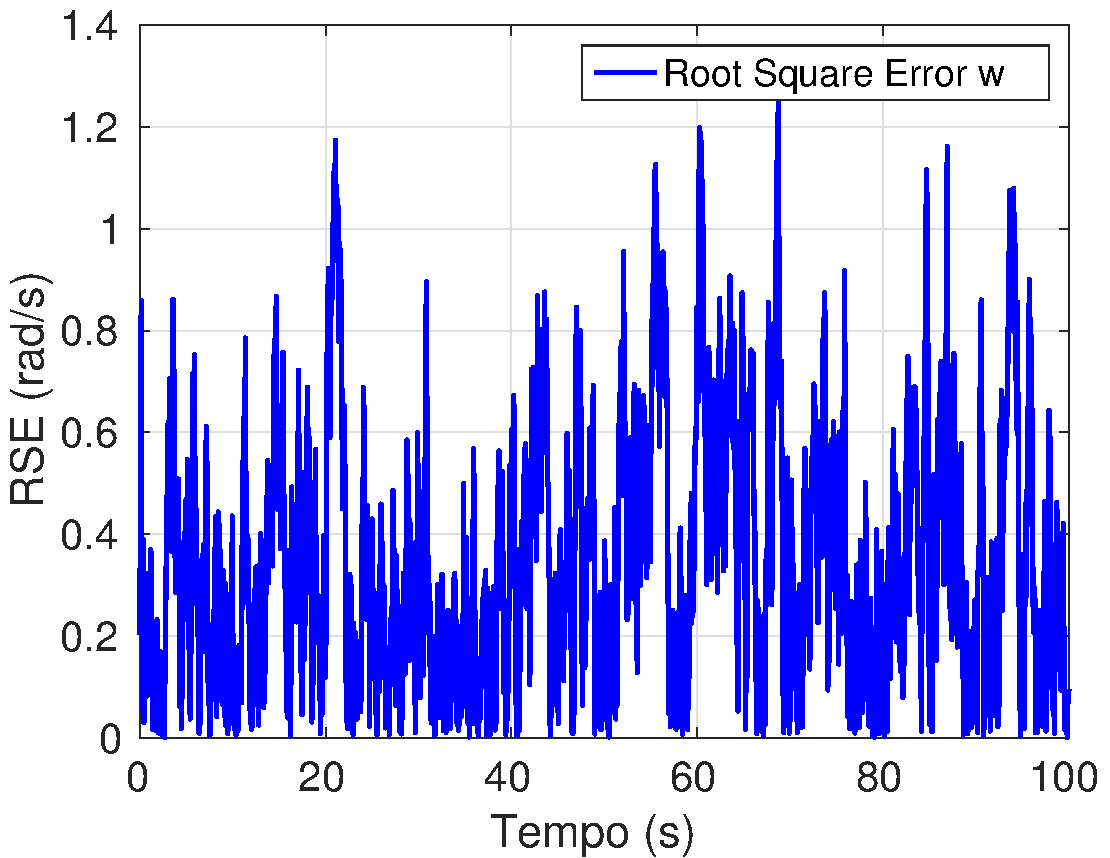
\includegraphics[width=0.45\textwidth]{RSE-w.pdf}
    }
    \caption{Trajetórias e Root Square Error em $x$, $y$, $\psi$, $v$ e $w$ - Tracking adversário}
    \label{estatisticas_adversario}
  \end{figure}
  

  
Para o cálculo dos erros quadráticos médios da estimativa e da observação para o tracking do robô adversário, a fim de comparação entre eles e avaliação do desempenho do filtro, a simulação descrita acima foi repetida 500 vezes, computando-se então a média dos erros médios das 500 simulações. Os resultados seguem na Tabela \ref{estatisticas1}. As velocidades linear e angular segundo os dados da visão foram calculadas por derivação numérica, empregando os valores de $x$ e $y$ observados em duas iterações consecutivas.

\begin{table}[!t]
%% increase table row spacing, adjust to taste
%\renewcommand{\arraystretch}{1.8}
% if using array.sty, it might be a good idea to tweak the value of
% \extrarowheight as needed to properly center the text within the cells
\caption{RMSE - Tracking adversário}
\label{estatisticas1}
\centering
% Some packages, such as MDW tools, offer better commands for making tables
% than the plain LaTeX2e tabular which is used here.
\begin{tabular}{|c|c|c|c|} 
%\hline
%\multicolumn{4}{|c|}{Erro Quadrático Médio}
\hline
\multicolumn{2}{|c|}{Estimativa} & \multicolumn{2}{|c|}{Observação}\\
\hline
$x$ & $0.2433$ & $x$ & $0.3093$ \\
\hline
$y$ & $0.2431$ & $y$ & $0.3089$ \\
\hline
$\psi$ & $0.0631$ & $\psi$ & $0.0798$ \\
\hline
$v$ & $0.6468$ & $v$ & $19.9163$ \\
\hline
$w$ & $0.3795$ & $w$ & $4.1417$ \\
\hline
\end{tabular}
\end{table}

Para o tracking da bola, também foi empregada uma simulação de $100s$ e passo de $\frac{1}{30}s$. Os erros quadráticos médios também foram calculados considerando uma média com 500 simulações. Os resultados seguem na tabela \ref{estatisticas2} e os valores usados para $Q$ e $R$ seguem na tabela \ref{covariancias2}. Os resultados gráficos para uma simulação estão presentes nas figuras \ref{trajetorias2} e \ref{estatisticas_bola}.

% trajetórias  bola
\begin{figure}[!t]
\centering
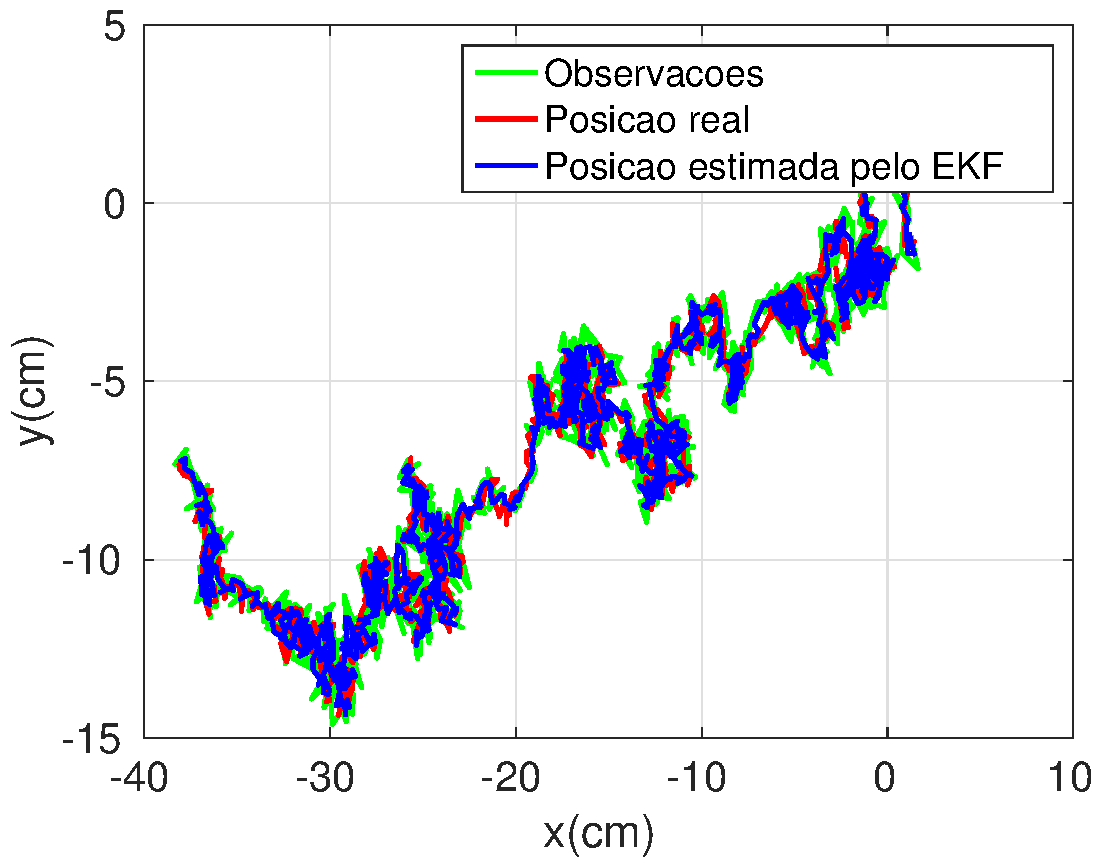
\includegraphics[width=2.5in]{trajetorias2.pdf}
\DeclareGraphicsExtensions.
\caption{Trajetórias simulação - Tracking bola}
\label{trajetorias2}
\end{figure}

% erros em x e y
 \begin{figure}[!ht]
    \subfloat[RSE-$x$\label{RSE-x2}]{%
      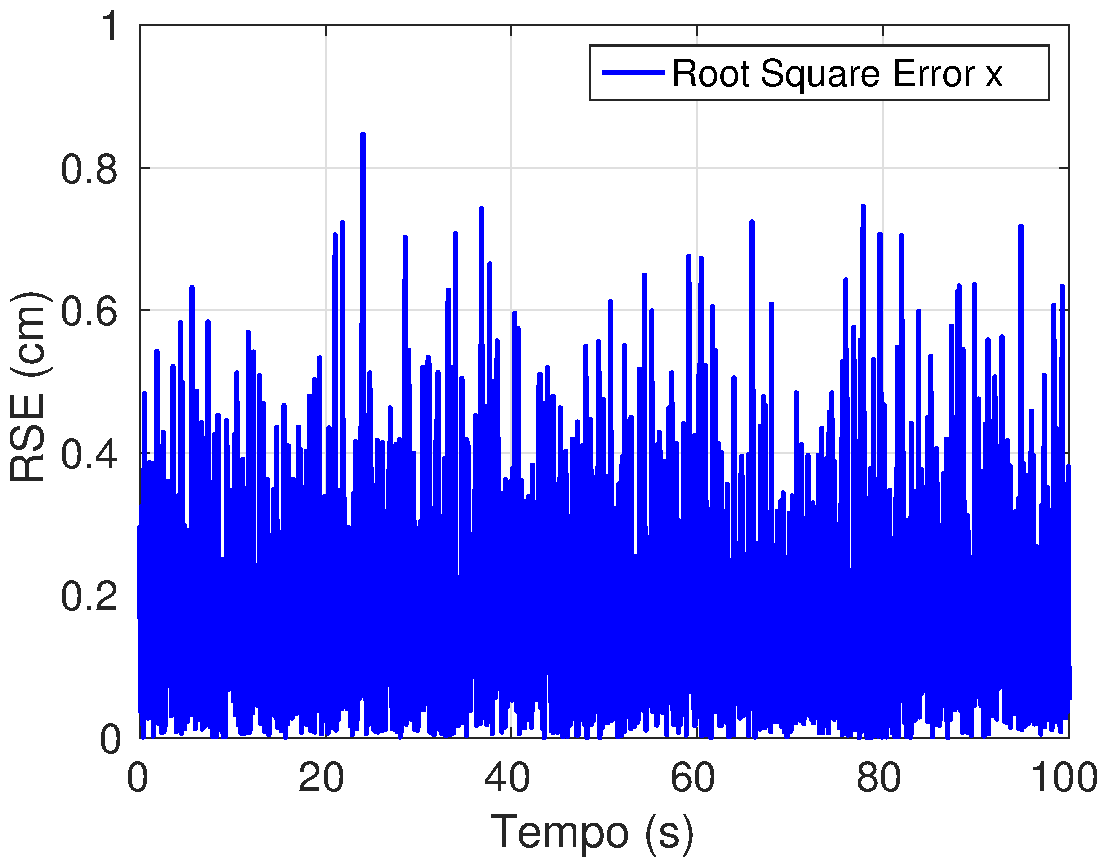
\includegraphics[width=0.45\textwidth]{RSE-x2.pdf}
    }
    \hfill
    \subfloat[RSE-$y$\label{RSE-y2}]{%
      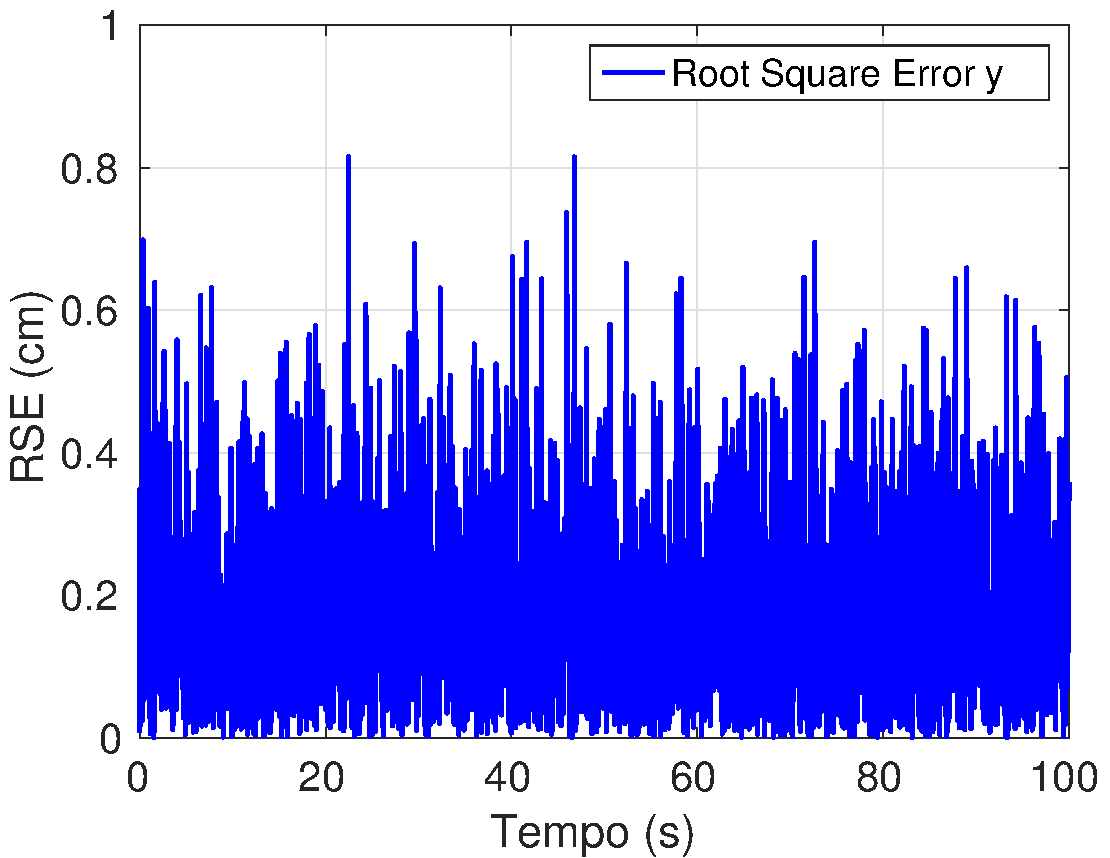
\includegraphics[width=0.45\textwidth]{RSE-y2.pdf}
    }
    \hfill
%    \caption{Root Square Error em $x$ e $y$ - Tracking bola}
%    \label{erros_xy2}
%  \end{figure}
% erros em vs e vy
% \begin{figure}[!ht]
    \subfloat[RSE-$v_x$\label{RSE-vx}]{%
      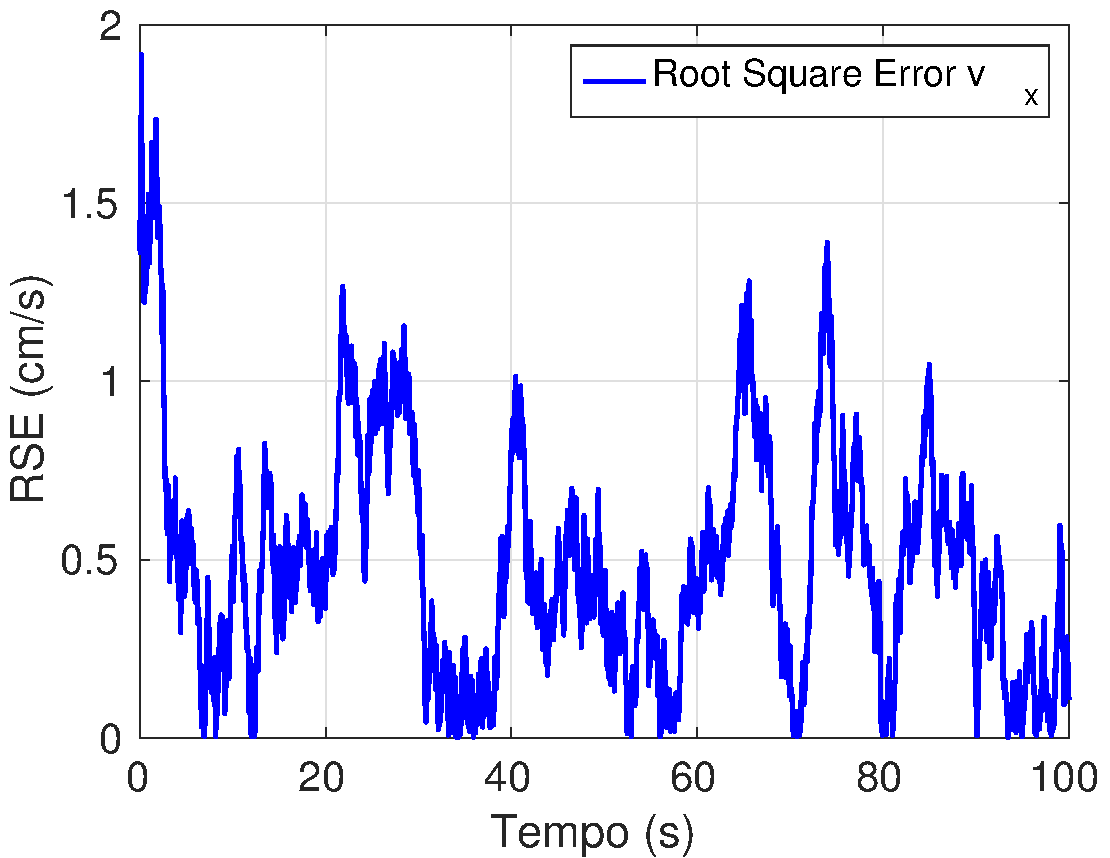
\includegraphics[width=0.45\textwidth]{RSE-v_x2.pdf}
    }
    \hfill
    \subfloat[RSE-$v_y$\label{RSE-vy}]{%
      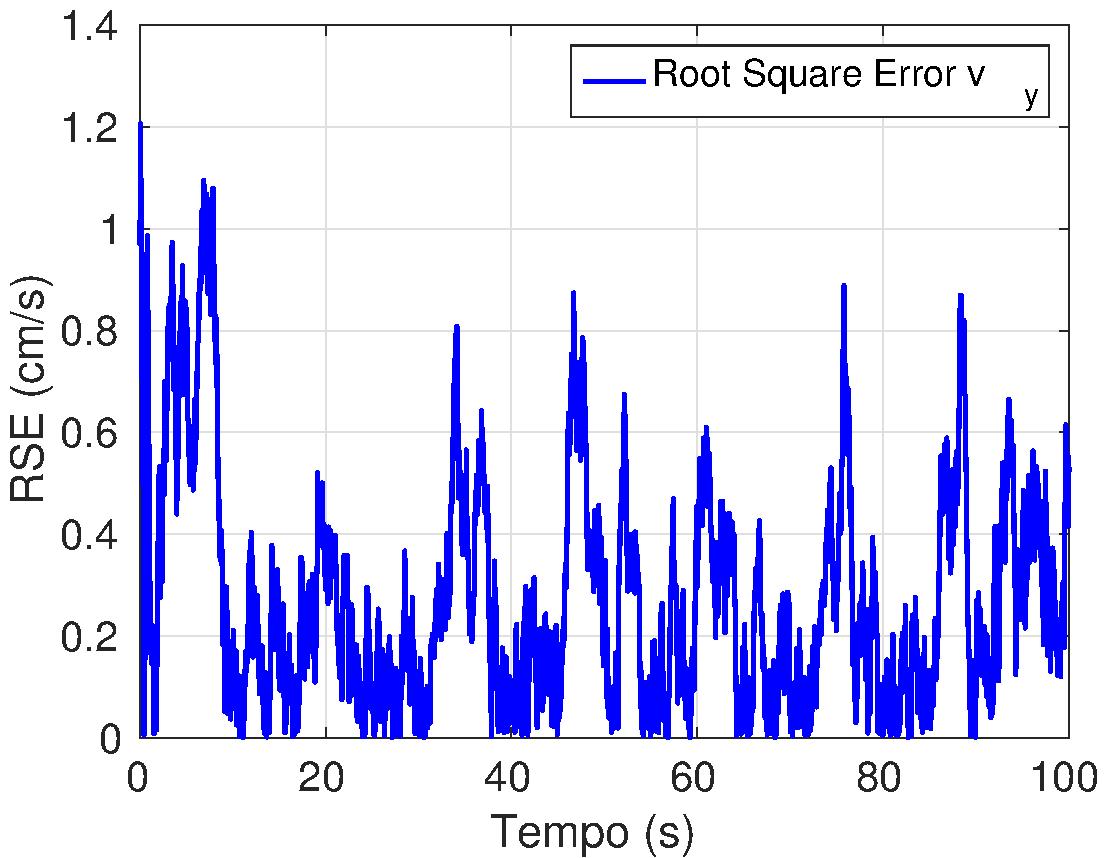
\includegraphics[width=0.45\textwidth]{RSE-v_y2.pdf}
    }
    \caption{Root Square Error em $x$, $y$, $v_x$ e $v_y$ - Tracking bola}
    \label{estatisticas_bola}
  \end{figure}

\begin{table}[!t]
\caption{Covariâncias - Tracking bola}
\label{covariancias2}
\centering
% Some packages, such as MDW tools, offer better commands for making tables
% than the plain LaTeX2e tabular which is used here.
\begin{tabular}{c} 
$Q = \begin{bmatrix} $0.05$ & $0$ & $0$ & $0$ \\ $0$ & $0.05$ & $0$ & $0$ \\ $0$ & $0$ & $1$ & $0$ \\ $0$ & $0$ & $0$ & $1$ \end{bmatrix}$\\
$R = \begin{bmatrix} $0.1$ & $0$ \\ $0$ & $0.1$ \end{bmatrix}$\\
\end{tabular}
\end{table}

\begin{table}[!t]
%% increase table row spacing, adjust to taste
%\renewcommand{\arraystretch}{1.8}
% if using array.sty, it might be a good idea to tweak the value of
% \extrarowheight as needed to properly center the text within the cells
\caption{RMSE - Tracking bola}
\label{estatisticas2}
\centering
% Some packages, such as MDW tools, offer better commands for making tables
% than the plain LaTeX2e tabular which is used here.
\begin{tabular}{|c|c|c|c|} 
%\hline
%\multicolumn{4}{|c|}{Erro Quadrático Médio}
\hline
\multicolumn{2}{|c|}{Estimativa} & \multicolumn{2}{|c|}{Observação}\\
\hline
$x$ & $0.1788$ & $x$ & $0.2523$ \\
\hline
$y$ & $0.1788$ & $y$ & $0.2521$ \\
\hline
$v_x$ & $0.3915$ & $v_x$ & $11.9652$\\
\hline
$v_y$ & $0.3863$ & $v_y$ & $11.9559$\\
\hline
\end{tabular}
\end{table}

Os valores empregados para as matrizes de covariância são apenas estimativas por enquanto, posteriormente planeja-se tirar um modelo mais preciso dos erros do movimento e da observação da câmera. A estimativa foi feita supondo um erro médio de aproximadamente $0.3cm$ em $x$ e $y$ e 5 graus em $\psi$ para os dados da visão, além de considerar uma variância bem alta para as acelerações.

Analisando os resultados, é possível constatar que o filtro de Kalman ofereceu um bom ganho de precisão em relação à observação. O erro médio da estimativa é de aproximadamente 78\% do erro da visão, para o tracking do adversário, e de 70\% para o tracking da bola. Além disso, o filtro fornece uma boa estimativa do valor das velocidades, linear e angular, o que não é possível alcançar só com a derivação numérica da posição com a informação da câmera, como percebe-se nos valores revelados nas tabelas \ref{estatisticas1} e \ref{estatisticas2}. Observa-se também pelas figuras \ref{estatisticas_adversario}, \ref{trajetorias2} e \ref{estatisticas_bola} que o filtro mantém sempre o rastreio do objeto, e o erro quadrático não diverge em nenhum momento.

\section{Conclusão}

Através do estudo realizado, foi possível conhecer bem os principais filtros bayesianos empregados para problemas de tracking e localização global em robótica, assim como implementá-los em problemas de localização genéricos com linguagem de alto nível e entender suas aplicações e particularidades.

Para o desafio desse projeto, que consiste em rastrear e estimar as velocidades de robôs diferenciais e da bola na competição IEEE’s Very Small Size Soccer (VSS), constatou-se a utilidade e aplicação dessas técnicas, em especial o filtro de Kalman extendido, uma extensão não linear do Filtro de Kalman. O resultado obtido através da simulação em MATLAB do problema com essa técnica de filtragem revelou um bom desempenho, mostrando sua eficácia em obter uma boa estimativa da posição do objeto e de suas velocidades linear e angular.

Tendo em vista esse resultado positivo, o próximo objetivo é aplicar a técnica explicada em robôs reais, utilizando um time de 3 robôs e câmera, além de integrar ao código principal da equipe ITAndrois. Além disso, espera-se também obter no futuro melhores estimativas para as covariâncias e parâmetros empregados, utilizando experimentos e técnicas de identificação de sistemas.

\section{Plano de Trabalho e Cronograma Futuro}
\textbf{março/abril}
\begin{itemize}
    \item Implementação do filtro no sistema embarcado do robô
    \item Criação de ferramentas de teste e análise do desempenho do código.
\end{itemize}
\textbf{maio/junho}
\begin{itemize}
    \item Testes no robô
    \item Otimização de parâmetros do filtro
\end{itemize}
\textbf{julho}
\begin{itemize}
    \item Integração com o código do time da ITAndroids
    \item Testes no robô
    \item Confecção do relatório final
\end{itemize}
% conference papers do not normally have an appendix


% use section* for acknowledgment
\section{Agradecimentos}
Agradeço ao CNPQ, por prover ajuda financeira para realizar esse projeto. Agradeço à ITAndroids, por compartilhar conhecimento e ferramentas que tornam esse projeto possível.





% trigger a \newpage just before the given reference
% number - used to balance the columns on the last page
% adjust value as needed - may need to be readjusted if
% the document is modified later
%\IEEEtriggeratref{8}
% The "triggered" command can be changed if desired:
%\IEEEtriggercmd{\enlargethispage{-5in}}

% references section

% can use a bibliography generated by BibTeX as a .bbl file
% BibTeX documentation can be easily obtained at:
% http://mirror.ctan.org/biblio/bibtex/contrib/doc/
% The IEEEtran BibTeX style support page is at:
% http://www.michaelshell.org/tex/ieeetran/bibtex/
%\bibliographystyle{IEEEtran}
% argument is your BibTeX string definitions and bibliography database(s)
%\bibliography{IEEEabrv,../bib/paper}
%\usepackage[backend=bibtex,style=ieee,sorting=none]{biblatex}
%\bibliography{main.bib}
\section{Bibliografia}
%\bibliographystyle{IEEEtran}
%\bibliographystyle{bibstyle}
\printbibliography[heading=none]
%
% <OR> manually copy in the resultant .bbl file
% set second argument of \begin to the number of references
% (used to reserve space for the reference number labels box)
%\section{Bibliografia}
%\begin{thebibliography}{1}

%\bibitem{P.Robotics}
%Thrun, S., Burgard, W., Fox, D.: Probabilistic Robotics. MIT Press. 2005

%\bibitem{Simo_bayesianFiltering}
%Särkkä (2013). Bayesian Filtering and Smoothing. Cambridge University Press.

%\bibitem{Optimal_Filtering}
%Anderson, B., D., O., Moore, J., B.: Optimal Filtering. Prentice-Hall, Inc., Englewood Cliffs, N.J. 1979

%\bibitem{unscented_filtering}
%Julier, S. and Uhlmann, J. (2004). Unscented filtering and nonlinear estimation. Proceedings of the IEEE 92(3): 401-422.

%\bibitem{ukf} 
%Wan, E. A. and Merwe, R. V. D. (2000). The unscented kalman filter for nonlinear estimation, pp.153-158.

%\bibitem{monte_carlo_localization}
%Dellaert, F., Fox, D., Burgard, W., Thrun, S. 1999. Monte Carlo Localization for mobile robots. In ICRA

%\end{thebibliography}
% that's all folks
\end{document}

